\documentclass[11pt,a4paper]{article}
\usepackage[T1]{fontenc}
\usepackage[utf8]{inputenc}
\usepackage{lmodern}
\usepackage{textcomp}
\usepackage[left=1.8cm,right=1.8cm,top=2.3cm,bottom=2.2cm,headheight=14pt,headsep=8pt]{geometry}
\usepackage{multicol}
\usepackage{xcolor}
\usepackage{fancyhdr}
\usepackage{graphicx}
\usepackage{array}
\usepackage{amsmath,amssymb}
\usepackage{setspace}
\usepackage{longtable}
\graphicspath{{../}}
\definecolor{ygreen}{RGB}{46,139,87}
\renewcommand{\normalsize}{\fontsize{10.9}{13.4}\selectfont}
\renewcommand{\familydefault}{\rmdefault}
\setlength{\parindent}{0pt}
\setlength{\columnsep}{0.8cm}
\setlength{\columnseprule}{0.4pt}
\setlength{\multicolsep}{3pt plus 1pt minus 1pt}
\renewcommand{\textsubscript}[1]{\ensuremath{_{\text{\fontsize{8}{8}\selectfont #1}}}}
\renewcommand{\textsuperscript}[1]{\ensuremath{^{\text{\fontsize{8}{8}\selectfont #1}}}}
\newcommand{\qn}[1]{\textbf{\fontsize{11.5}{13}\selectfont #1}}
\newcommand{\qsep}{\par\vspace{1pt}\noindent\rule{0pt}{0.4pt}\par\vspace{5pt}}
\newcommand{\fwrule}{\par\vspace{5pt}\noindent\rule{\linewidth}{1.4pt}\par\vspace{7pt}}
\newsavebox{\fitb}
\newcommand{\fitbox}[1]{\sbox{\fitb}{#1}\ifdim\wd\fitb>\linewidth\resizebox{\linewidth}{!}{\usebox{\fitb}}\else\usebox{\fitb}\fi}
\newcommand{\diqqat}[1]{\par\smallskip\noindent\textbf{Diqqat!} #1\par\medskip}
\newcommand{\javob}{\par\smallskip\noindent\textbf{Javob:} \rule[-2pt]{7.5cm}{0.4pt}\par\smallskip\noindent\textbf{Diqqat!} Javobingizni javoblar varaqasiga ko`chirib yozing.\par\medskip}
\pagestyle{fancy}
\fancyhf{}
\renewcommand{\headrulewidth}{0.4pt}
\fancyhead[L]{\textit{Milliy sertifikat 2026. Kimyo}}
\fancyhead[R]{20-variant}
\fancyfoot[L]{\fontsize{8}{9}\selectfont \textcopyright{} Colba maktabi, 2026}
\fancyfoot[C]{\thepage}
\fancypagestyle{first}{\fancyhf{}\renewcommand{\headrulewidth}{0pt}\fancyfoot[L]{\fontsize{8}{9}\selectfont \textcopyright{} Colba maktabi, 2026}\fancyfoot[C]{\thepage}}
\begin{document}
\normalsize
\thispagestyle{first}
\noindent\fcolorbox{ygreen}{white}{\parbox{\dimexpr\linewidth-2\fboxsep-2\fboxrule\relax}{%
\textbf{\fontsize{13}{15}\selectfont Nazorat testi}\ \textit{\fontsize{10}{12}\selectfont $\cdot$ Aralash test $\cdot$ 20-variant}\hfill
\begin{tabular}[t]{@{}r@{}}\textit{Milliy sertifikat 2026. Kimyo}\\ \textbf{\textit{\fontsize{8}{9}\selectfont Vaqt:}} \textit{\fontsize{10}{12}\selectfont 180 daqiqa}\end{tabular}}}
\par\medskip
\noindent\textit{Davriy jadvaldan foydalanish mumkin.}
\par\medskip
\begin{multicols}{2}
\noindent\qn{1.} 1 g He 127 \textdegree{}C va 1 atm bosimda qancha hajm (l) egallaydi? (R = 0,082 l$\cdot$atm/(mol$\cdot$K))

\noindent A)~\textsl{8,2} \hfill B)~\textsl{16,4} \hfill C)~\textsl{4,1} \hfill D)~\textsl{5,6}\par
\qsep
\noindent\qn{2.} Quyidagi tuzlarning qaysilari suvli eritmasi kislotali muhitga ega? 1) NH\textsubscript{4}Cl; 2) KNO\textsubscript{3}; 3) FeCl\textsubscript{3}; 4) Na\textsubscript{2}SO\textsubscript{4}

\noindent A)~\textsl{2} \hfill B)~\textsl{1, 2} \hfill C)~\textsl{2, 3, 4} \hfill D)~\textsl{1, 3}\par
\qsep
\noindent\qn{3.} Quyidagilarni jism va moddalarga ajrating: mix, qaychi, etanol, alyuminiy, kislorod, osh tuzi. Ulardan nechtasi modda?

\noindent A)~\textsl{4} \hfill B)~\textsl{5} \hfill C)~\textsl{3} \hfill D)~\textsl{2}\par
\qsep
\noindent\qn{4.} Jadvalda bog`lar hosil qiluvchi atomlarning elektrmanfiyliklari berilgan:
\begin{center}
\renewcommand{\arraystretch}{1.15}
\fitbox{\begin{tabular}{|c|c|c|}\hline
\textbf{Bog`} & \textbf{EM (1-atom)} & \textbf{EM (2-atom)} \\ \hline
Na--Cl & 0,9 & 3 \\ \hline
N--H & 3 & 2,1 \\ \hline
H--F & 2,1 & 4 \\ \hline
Mg--O & 1,2 & 3,5 \\ \hline
\end{tabular}}
\end{center}
Qaysi bog` eng qutbli (eng ko`p ionli xarakterga ega)?

\noindent A)~\textsl{Na--Cl} \hfill B)~\textsl{N--H} \hfill C)~\textsl{Mg--O} \hfill D)~\textsl{H--F}\par
\qsep
\noindent\qn{5.} 3 mol AlCl\textsubscript{3} va 2 mol HNO\textsubscript{3} suvda eritilib, eritma hajmi 5 l ga yetkazildi. Eritmadagi barcha ionlarning umumiy molyar \textbf{konsentratsiyasini (mol/l) aniqlang} (kuchli elektrolitlar to`liq dissotsilanadi).

\noindent A)~\textsl{1} \hfill B)~\textsl{6,4} \hfill C)~\textsl{3,2} \hfill D)~\textsl{1,6}\par
\qsep
\noindent\qn{6.} 2SO\textsubscript{2} + O\textsubscript{2} $\rightleftarrows$ 2SO\textsubscript{3} reaksiyasida SO\textsubscript{2} va O\textsubscript{2} stexiometrik nisbatda olingan umumiy 12 mol aralashma muvozanat qaror topganda doimiy T va \textit{V} da bosim 25\% ga kamaydi. Muvozanatdagi SO\textsubscript{3} ning \textbf{miqdorini (mol) aniqlang.}

\noindent A)~\textsl{2} \hfill B)~\textsl{1} \hfill C)~\textsl{6} \hfill D)~\textsl{3}\par
\qsep
\noindent\qn{7.} 1 mol C\textsubscript{2}H\textsubscript{6} tarkibida necha mol atom bor?

\noindent A)~\textsl{7} \hfill B)~\textsl{8} \hfill C)~\textsl{9} \hfill D)~\textsl{1}\par
\qsep
\noindent\qn{8.} Quyidagi zarrachalardan qaysilari neon atomi bilan izoelektron? 1) O\textsuperscript{2$-$}; 2) Mg\textsuperscript{2+}; 3) Ca\textsuperscript{2+}; 4) K\textsuperscript{+}

\noindent A)~\textsl{1, 2, 4} \hfill B)~\textsl{2, 3, 4} \hfill C)~\textsl{1, 2} \hfill D)~\textsl{1, 3}\par
\qsep
\noindent\qn{9.} Grafikda tuzning eruvchanligi (g/100 g suv) haroratga bog`liq ko`rsatilgan.
\begin{center}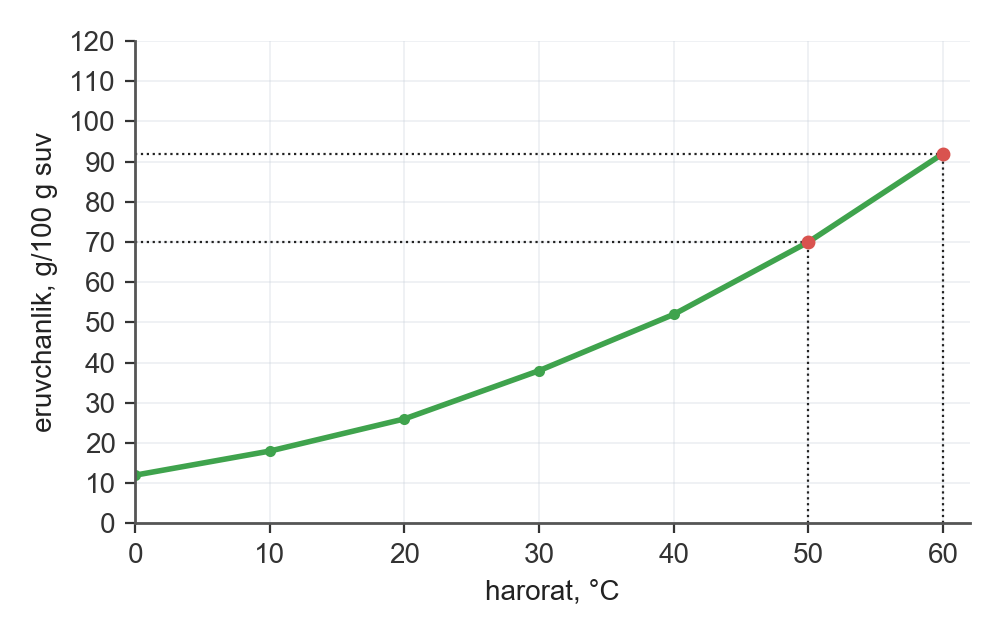
\includegraphics[width=0.86\linewidth]{rasmlar/gen/sol_v20_0.png}\end{center}
60 \textdegree{}C da tuzning to`yingan eritmasidagi massa \textbf{ulushini (\%) aniqlang.}

\noindent A)~\textsl{47,9} \hfill B)~\textsl{92} \hfill C)~\textsl{24} \hfill D)~\textsl{41,2}\par
\qsep
\noindent\qn{10.} Laboratoriyada KNO\textsubscript{3} eritmalari quyidagicha tayyorlangan:
\begin{center}
\renewcommand{\arraystretch}{1.15}
\fitbox{\begin{tabular}{|c|c|c|}\hline
\textbf{Idish} & \textbf{Eritma massasi, g} & \textbf{$\omega$(KNO\textsubscript{3}), \%} \\ \hline
A & 200 & 20 \\ \hline
B & 300 & 35 \\ \hline
\end{tabular}}
\end{center}
Bu ikki eritma bir idishga quyilib, yangi eritmadagi KNO\textsubscript{3} ning massa ulushi (\%) qancha bo`ladi?

\noindent A)~\textsl{27,5} \hfill B)~\textsl{55} \hfill C)~\textsl{26} \hfill D)~\textsl{29}\par
\qsep
\noindent\qn{11.} N\textsubscript{2} gazining 27 \textdegree{}C va 4 atm bosimdagi \textbf{zichligini (g/l) aniqlang.} (R = 0,082 l$\cdot$atm/(mol$\cdot$K))

\noindent A)~\textsl{9,11} \hfill B)~\textsl{4,55} \hfill C)~\textsl{2,28} \hfill D)~\textsl{1,25}\par
\qsep
\noindent\qn{12.} Rasmda davriy jadvalning bir qismi berilgan (\textit{X}, \textit{Y}, \textit{Z} --- noma'lum elementlar).
\begin{center}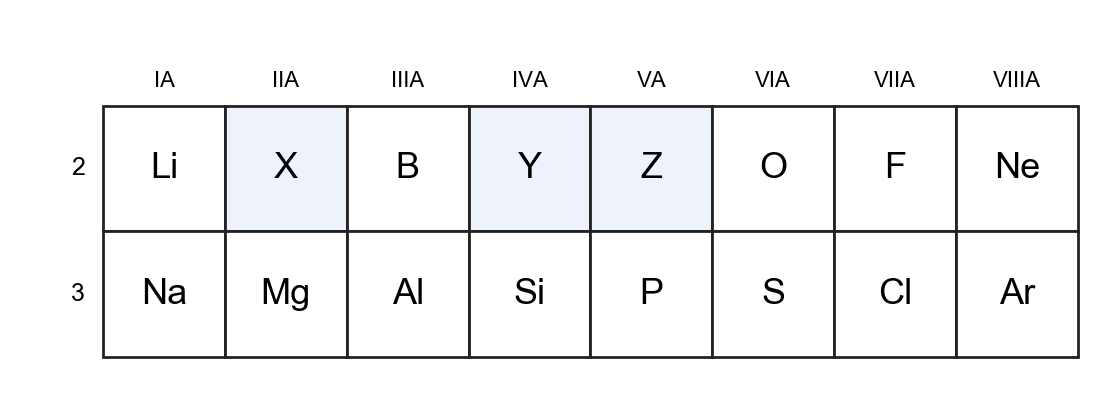
\includegraphics[width=0.86\linewidth]{rasmlar/gen/pt_580869.png}\end{center}
\textit{X}, \textit{Y}, \textit{Z} elementlardan qaysi birining elektrmanfiyligi eng katta?

\noindent\begin{tabular}{@{}p{0.47\linewidth}@{}p{0.47\linewidth}@{}}
A)~\textsl{\textit{X}} & B)~\textsl{\textit{Z}} \\
C)~\textsl{\textit{Y}} & D)~\textsl{uchalasiniki teng} \\
\end{tabular}\par
\qsep
\noindent\qn{13.} AgNO\textsubscript{3} ning suvli eritmasi inert elektrodlar bilan elektroliz qilinganda qaysi moddalar ajraladi?

\noindent\begin{tabular}{@{}p{0.47\linewidth}@{}p{0.47\linewidth}@{}}
A)~\textsl{Cu va Cl\textsubscript{2}} & B)~\textsl{Ag va O\textsubscript{2}} \\
C)~\textsl{H\textsubscript{2}, Cl\textsubscript{2} va NaOH} & D)~\textsl{Zn, H\textsubscript{2} va O\textsubscript{2}} \\
\end{tabular}\par
\qsep
\noindent\qn{14.} Ishqoriy metallar haqida qaysi fikrlar to`g`ri? 1) KOH -- kuchli ishqor; 2) Natriyning olinishi suyuqlanma NaCl elektrolizi bilan; 3) Natriy atomining tashqi qavatida 2 ta elektron bor; 4) Natriy suv bilan reaksiyada H\textsubscript{2} va NaOH hosil qiladi

\noindent A)~\textsl{1, 2, 4} \hfill B)~\textsl{2, 4} \hfill C)~\textsl{1, 2} \hfill D)~\textsl{2, 3}\par
\qsep
\noindent\qn{15.} Alyuminiy va mis dan iborat 14,5 g aralashma mo`l NaOH eritmasida eritilganda 10,08 l (n.sh.) gaz ajraldi. Aralashmadagi mis ning massa \textbf{ulushini (\%) aniqlang.}

\noindent A)~\textsl{55,9} \hfill B)~\textsl{44,1} \hfill C)~\textsl{22,1} \hfill D)~\textsl{50,3}\par
\qsep
\noindent\qn{16.} D-metallar va ularning birikmalari haqida qaysi fikrlar to`g`ri? 1) Temir sovuq konsentrlangan HNO\textsubscript{3} da passivlanadi; 2) Mis nam havoda (CuOH)\textsubscript{2}CO\textsubscript{3} qoplamasi bilan qoplanadi; 3) Cr\textsubscript{2}O\textsubscript{3} asosli oksid; 4) Zn(OH)\textsubscript{2} amfoter xossaga ega

\noindent A)~\textsl{1, 2, 4} \hfill B)~\textsl{3, 4} \hfill C)~\textsl{1, 2} \hfill D)~\textsl{2, 3}\par
\qsep
\noindent\qn{17.} Reaksiya tenglamasi: CaSO\textsubscript{4} + Na\textsubscript{2}CO\textsubscript{3} $\to$ CaCO\textsubscript{3} + Na\textsubscript{2}SO\textsubscript{4}. Reaksiyaga tarkibida 75\% aralashma bo`lgan 136 g namuna (asosiy modda CaSO\textsubscript{4}) kirishdi. Na\textsubscript{2}SO\textsubscript{4} \textbf{massasini (g) hisoblang.}

\noindent A)~\textsl{71} \hfill B)~\textsl{17,75} \hfill C)~\textsl{53,25} \hfill D)~\textsl{35,5}\par
\qsep
\noindent\qn{18.} Al\textsubscript{2}O\textsubscript{3} + 3H\textsubscript{2}SO\textsubscript{4} $\to$ Al\textsubscript{2}(SO\textsubscript{4})\textsubscript{3} + 3H\textsubscript{2}O jarayoni uchun 9,8 g H\textsubscript{2}SO\textsubscript{4} olingan. Al\textsubscript{2}O\textsubscript{3} \textbf{massasini (g) aniqlang.}

\noindent A)~\textsl{30,6} \hfill B)~\textsl{6,8} \hfill C)~\textsl{3,4} \hfill D)~\textsl{1,7}\par
\qsep
\noindent\qn{19.} 2Al + 3CuCl\textsubscript{2} $\to$ 2AlCl\textsubscript{3} + 3Cu reaksiyasida 5,4 g Al ishtirok etdi. Cu \textbf{massasini (g) toping.}

\noindent A)~\textsl{8,53} \hfill B)~\textsl{38,4} \hfill C)~\textsl{9,6} \hfill D)~\textsl{19,2}\par
\qsep
\noindent\qn{20.} 2C\textsubscript{2}H\textsubscript{6} + 7O\textsubscript{2} $\to$ 4CO\textsubscript{2} + 6H\textsubscript{2}O jarayoni uchun 2,24 l (n.sh.) C\textsubscript{2}H\textsubscript{6} olingan (unum 75\%). CO\textsubscript{2} \textbf{massasini (g) aniqlang.}

\noindent A)~\textsl{2,2} \hfill B)~\textsl{13,2} \hfill C)~\textsl{6,6} \hfill D)~\textsl{3,3}\par
\qsep
\noindent\qn{21.} Alken, alkadiyen va alkinlar haqida qaysi fikrlar to`g`ri? 1) Etilen sanoatda kreking gazlaridan olinadi; 2) Propenga HBr birikishi Markovnikov qoidasiga bo`ysunadi; 3) Asetilenni Kucherov reaksiyasi bilan sirka aldegidiga aylantirish mumkin; 4) Etilen bromli suvni rangsizlantiradi

\noindent\begin{tabular}{@{}p{0.47\linewidth}@{}p{0.47\linewidth}@{}}
A)~\textsl{1, 2, 3, 4} & B)~\textsl{1, 2, 4} \\
C)~\textsl{1, 3, 4} & D)~\textsl{2, 3, 4} \\
\end{tabular}\par
\qsep
\noindent\qn{22.} Arenlar, neft va tabiiy gaz haqida qaysi fikrlar to`g`ri? 1) Tabiiy gazning asosiy qismi propan; 2) Benzoldan nitrobenzol nitrolash bilan olinadi; 3) Benzol bromli suvni rangsizlantirmaydi; 4) Benzolda 6 ta sp\textsuperscript{2} gibridlangan uglerod bor

\noindent A)~\textsl{3, 4} \hfill B)~\textsl{1, 3, 4} \hfill C)~\textsl{1, 2, 3} \hfill D)~\textsl{2, 3, 4}\par
\qsep
\noindent\qn{23.} 2C\textsubscript{2}H\textsubscript{5}OH + 2Na $\to$ 2C\textsubscript{2}H\textsubscript{5}ONa + H\textsubscript{2} reaksiyasida 4,6 g C\textsubscript{2}H\textsubscript{5}OH ishtirok etdi. H\textsubscript{2} \textbf{miqdorini (mol) toping.}

\noindent A)~\textsl{0,05} \hfill B)~\textsl{0,2} \hfill C)~\textsl{0,1} \hfill D)~\textsl{0,03}\par
\qsep
\noindent\qn{24.} 44 g CH\textsubscript{3}CHO dan quyidagi ikki bosqichda CH\textsubscript{3}COOC\textsubscript{2}H\textsubscript{5} olinadi: 1) CH\textsubscript{3}CHO + Ag\textsubscript{2}O $\to$ CH\textsubscript{3}COOH + 2Ag (unum 80\%); 2) CH\textsubscript{3}COOH + C\textsubscript{2}H\textsubscript{5}OH $\to$ CH\textsubscript{3}COOC\textsubscript{2}H\textsubscript{5} + H\textsubscript{2}O (unum 80\%). Oxirgi mahsulot CH\textsubscript{3}COOC\textsubscript{2}H\textsubscript{5} ning \textbf{massasini (g) toping.}

\noindent A)~\textsl{70,4} \hfill B)~\textsl{88} \hfill C)~\textsl{112,64} \hfill D)~\textsl{56,32}\par
\qsep
\noindent\qn{25.} Karbon kislotalar haqida qaysi fikrlar to`g`ri? 1) Stearin kislota to`yinmagan kislota; 2) Sirka angidrid ikki molekula sirka kislotadan suv chiqib hosil bo`ladi; 3) Sirka kislota karbonatlar bilan CO\textsubscript{2} ajratadi; 4) Karboksil guruh karbonil va gidroksil guruhlardan iborat

\noindent A)~\textsl{1, 3} \hfill B)~\textsl{2, 3, 4} \hfill C)~\textsl{1, 3, 4} \hfill D)~\textsl{1, 2, 3}\par
\qsep
\noindent\qn{26.} Murakkab efirlar va yog`lar haqida qaysi fikrlar to`g`ri? 1) Dietil efir spirtdan yuqori haroratda qaynaydi; 2) Efirlanish reaksiyasi qaytmas; 3) Yog`lar glitserin va yuqori yog` kislotalarning murakkab efirlari; 4) Suyuq yog`lar to`yinmagan kislotalardan hosil bo`lgan

\noindent A)~\textsl{1, 3} \hfill B)~\textsl{1, 4} \hfill C)~\textsl{3, 4} \hfill D)~\textsl{2, 3, 4}\par
\qsep
\noindent\qn{27.} Uglevodlar haqida qaysi fikrlar to`g`ri? 1) Glyukoza "kumush ko`zgu" reaksiyasini beradi; 2) Fruktoza ketospirt; 3) Kraxmal yod bilan ko`k rang beradi; 4) Selluloza $\beta$-glyukoza qoldiqlaridan iborat

\noindent\begin{tabular}{@{}p{0.47\linewidth}@{}p{0.47\linewidth}@{}}
A)~\textsl{1, 2, 4} & B)~\textsl{1, 2, 3, 4} \\
C)~\textsl{1, 3, 4} & D)~\textsl{1, 2, 3} \\
\end{tabular}\par
\qsep
\noindent\qn{28.} Aminlar, aminokislotalar va oqsillar haqida qaysi fikrlar to`g`ri? 1) Aminlar kuchsiz asoslar xossasini namoyon qiladi; 2) Aminokislotalar faqat kislotali xossaga ega; 3) Aminokislotalar amfoter birikmalar; 4) Dipeptidda 2 ta peptid bog` bor

\noindent A)~\textsl{2} \hfill B)~\textsl{1, 3} \hfill C)~\textsl{1, 4} \hfill D)~\textsl{3, 4}\par
\qsep
\noindent\qn{29.} Stirol monomeridan olingan polimerning polimerlanish darajasi 2500 bo`lsa, uning molyar \textbf{massasini (g/mol) aniqlang.}

\noindent A)~\textsl{130000} \hfill B)~\textsl{520000} \hfill C)~\textsl{2604} \hfill D)~\textsl{260000}\par
\qsep
\noindent\qn{30.} Laboratoriyada karbonat angidrid olish uchun qaysi moddalar ishlatiladi?
\noindent A)~\textsl{C\textsubscript{2}H\textsubscript{5}OH + H\textsubscript{2}SO\textsubscript{4} (kons.), 170 \textdegree{}C}\par
\noindent B)~\textsl{KMnO\textsubscript{4} (qizdirish)}\par
\noindent C)~\textsl{Zn + HCl}\par
\noindent D)~\textsl{CaCO\textsubscript{3} + HCl}\par
\qsep
\noindent\qn{31.} Rasmda laboratoriyada gaz olish asbobi ko`rsatilgan. Qaysi moddalar o`zaro ta'sirlashadi?
\begin{center}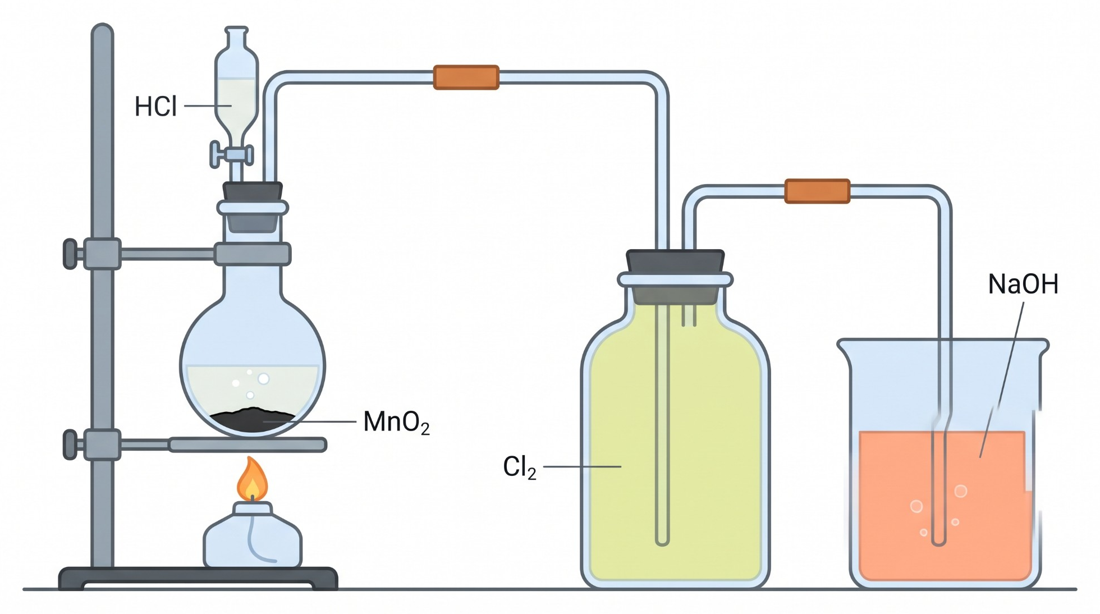
\includegraphics[width=0.86\linewidth]{rasmlar/darslik/d_xlor.png}\end{center}
\noindent A)~\textsl{MnO\textsubscript{2} va konsentrlangan HCl}\par
\noindent B)~\textsl{Zn va HCl}\par
\noindent C)~\textsl{CaCO\textsubscript{3} va HCl}\par
\noindent D)~\textsl{NH\textsubscript{4}Cl va Ca(OH)\textsubscript{2}}\par
\qsep
\noindent\qn{32.} Fenolftalein indikatori kislotali muhitda qanday rang beradi?
\noindent A)~\textsl{malina rangga kiradi (pushti)}\par
\noindent B)~\textsl{sariq}\par
\noindent C)~\textsl{rangsiz}\par
\noindent D)~\textsl{ko`k   ---}\par
\qsep
\end{multicols}
\medskip
\noindent\setlength{\fboxsep}{0pt}\fbox{\begin{tabular}{p{0.74\linewidth}|p{0.2\linewidth}}
\parbox[t]{0.72\linewidth}{\vspace{3pt}\textbf{Topshiriqlar (33--35) va javob variant (A--F)larini o`zaro to`g`ri moslashtiring.} Metan (CH\textsubscript{4}) va eten (C\textsubscript{2}H\textsubscript{4}) dan iborat 10,08 l (n.sh.) aralashma bromli suvdan o`tkazilganda 24 g brom yutildi.
\vspace{3pt}} & \parbox[t]{0.19\linewidth}{\vspace{3pt}A~\textsl{3,36}\\[3pt]
B~\textsl{1,68}\\[3pt]
C~\textsl{6,72}\\[3pt]
D~\textsl{112}\\[3pt]
E~\textsl{33,33}\\[3pt]
F~\textsl{26,67}}\\ \hline
\parbox[t]{0.72\linewidth}{\vspace{2pt}\textbf{33. Aralashmadagi eten (C\textsubscript{2}H\textsubscript{4}) hajmini (l, n.sh.) aniqlang.}\vspace{2pt}} & \\ \hline
\parbox[t]{0.72\linewidth}{\vspace{2pt}\textbf{34. Aralashmadagi eten (C\textsubscript{2}H\textsubscript{4}) hajmiy ulushini (\%) aniqlang.}\vspace{2pt}} & \\ \hline
\parbox[t]{0.72\linewidth}{\vspace{2pt}\textbf{35. Aralashmani to`liq yoqish uchun zarur havo hajmini (l, n.sh.; havoda 21\% kislorod bor) aniqlang.}\vspace{2pt}} & 
\end{tabular}}
\par\bigskip
\noindent\qn{36.} P + HNO\textsubscript{3} + H\textsubscript{2}O $\to$ H\textsubscript{3}PO\textsubscript{4} + NO reaksiya tenglamasini tenglang va barcha koeffitsiyentlar \textbf{yig`indisini aniqlang.}
\javob\qsep
\noindent\qn{37.} 5,6 g Fe reaksiyaga kirishdi (Fe + 2HCl $\to$ FeCl\textsubscript{2} + H\textsubscript{2}). Ajralgan H\textsubscript{2} \textbf{hajmini (l, n.sh.) hisoblang.}
\javob\qsep
\noindent\qn{38.} Alyuminiy va magniy dan iborat 12,9 g aralashma mo`l NaOH eritmasida eritilganda 10,08 l (n.sh.) gaz ajraldi. Aralashmadagi magniy ning massa \textbf{ulushini (\%) aniqlang.}
\javob\qsep
\noindent\qn{39.} C\textsubscript{3}H\textsubscript{7}OH va C\textsubscript{2}H\textsubscript{5}OH dan iborat 15,2 g aralashma natriy bilan to`liq reaksiyaga kirishganda ajraladigan vodorod \textbf{hajmini (l, n.sh.) toping.}
\javob\qsep
\noindent\qn{40.} Vinilxlorid monomeridan olingan polimerning polimerlanish darajasi 2500 bo`lsa, uning molyar \textbf{massasini (g/mol) aniqlang.}
\javob\qsep
\par\bigskip\begin{center}\textbf{\fontsize{13}{15}\selectfont YOZMA ISH}\end{center}
\noindent\qn{41.} \textbf{Topshiriqni bajarish jarayonida barcha reaksiya tenglamalarini yozing. Miqdoriy va arifmetik hisoblashlarni (unga asos bo`lgan usul yoki formulani ko`rsatgan holda) uzviy ketma-ketlikda bajaring.}\par\smallskip
Ketma-ket ulangan ikkita elektrolizyorda CuCl\textsubscript{2} va AgNO\textsubscript{3} eritmalari inert elektrodlar bilan elektroliz qilindi. Birinchi elektrolizyorning katodida 3,2 g Cu ajraldi (F = 96500 C/mol).\par
\noindent 1)Elektrolizyordan o`tgan zaryad miqdorini (C) hisoblang.\par
\noindent 2)Tok kuchi 5 A bo`lsa, elektroliz necha sekund davom etgan? O`tgan elektronlar miqdorini (mol) ham toping.\par
\noindent 3)Ikkinchi elektrolizyorning katodida ajralgan Ag massasini (g) aniqlang.\par
\noindent 4)Birinchi elektrolizyor anodida ajralgan gaz hajmini (l, n.sh.) toping. Ikkinchi elektrolizyor katodida ajralgan metallning miqdorini (mol) ham toping.\par
\noindent 5)Ikkala elektrolizyorda o`tgan elektronlar sonini (mol) taqqoslab, ularning teng ekanligini isbotlang. Agar tok kuchi 2 marta oshirilsa, shuncha zaryad o`tishi uchun necha sekund kerak?\par
\diqqat{Mazkur topshiriq kengaytirilgan javobni talab etib, uning yechilish usuli va shu usul asosidagi barcha hisoblash amallari javoblar varaqasida aks etishi lozim.}\qsep
\noindent\qn{42.} Quyidagi o`zgarishlar zanjirida \textit{X}, \textit{Y}, \textit{Z} noma'lum organik moddalar:\par
\[\setlength{\fboxsep}{0pt}\text{C\textsubscript{2}H\textsubscript{4}}\xrightarrow{\text{H\textsubscript{2}O, H\textsuperscript{+}}}\text{\textit{X}}\xrightarrow{\text{CuO, t\textdegree{}}}\text{\textit{Y}}\xrightarrow{\text{Ag\textsubscript{2}O, NH\textsubscript{3}}}\text{\textit{Z}}\xrightarrow{\text{C\textsubscript{2}H\textsubscript{5}OH, H\textsubscript{2}SO\textsubscript{4}}}\text{CH\textsubscript{3}COOC\textsubscript{2}H\textsubscript{5}}\]
\noindent 1)C\textsubscript{2}H\textsubscript{4} $\to$ \textit{X} : reaksiya tenglamasini yozing; hosil bo`lgan moddani nomlang.\par
\noindent 2)\textit{X} $\to$ \textit{Y} : reaksiya tenglamasini yozing; hosil bo`lgan moddani nomlang.\par
\noindent 3)\textit{Y} $\to$ \textit{Z} : reaksiya tenglamasini yozing; hosil bo`lgan moddani nomlang.\par
\noindent 4)\textit{Z} $\to$ CH\textsubscript{3}COOC\textsubscript{2}H\textsubscript{5} : reaksiya tenglamasini yozing; hosil bo`lgan moddani nomlang.\par
\diqqat{Mazkur topshiriq kengaytirilgan javobni talab etib, uning yechilish usuli va shu usul asosidagi barcha hisoblash amallari javoblar varaqasida aks etishi lozim.}\qsep
\noindent\qn{43.} \textbf{Topshiriqni bajarish jarayonida barcha reaksiya tenglamalarini yozing. Miqdoriy va arifmetik hisoblashlarni (unga asos bo`lgan usul yoki formulani ko`rsatgan holda) uzviy ketma-ketlikda bajaring.}\par\smallskip
Magniy (Mg) va alyuminiy (Al) dan iborat 6,45 g qotishma mo`l suyultirilgan sulfat kislotada eritildi, bunda 7,28 l (n.sh.) gaz ajraldi. Hosil bo`lgan eritmaga mo`l NaOH eritmasi qo`shildi, hosil bo`lgan cho`kma ajratib olindi va havoda qizdirib quritildi.\par
\noindent 1)Reaksiya tenglamalarini yozing va qotishmadagi har bir metallning massasini (g) aniqlang.\par
\noindent 2)Qotishmadagi Mg ning massa ulushini (\%) hisoblang.\par
\noindent 3)Eritish uchun sarflangan 20\% li H\textsubscript{2}SO\textsubscript{4} eritmasining massasini (g) aniqlang.\par
\noindent 4)Mo`l NaOH qo`shilganda hosil bo`lgan cho`kmaning formulasi va massasini (g) toping (reaksiya tenglamalarini yozing).\par
\noindent 5)Cho`kma havoda to`liq qizdirilganda hosil bo`lgan oksidning massasini (g) hisoblang.\par
\diqqat{Mazkur topshiriq kengaytirilgan javobni talab etib, uning yechilish usuli va shu usul asosidagi barcha hisoblash amallari javoblar varaqasida aks etishi lozim.}\qsep
\newpage
\noindent\textbf{\fontsize{13}{15}\selectfont Nazorat testi}\ \textit{$\cdot$ 20-variant}\hfill \textbf{Javoblar kaliti}\par\smallskip\hrule\smallskip
\textit{Faqat o`qituvchi uchun.}\par\medskip
\noindent\textbf{1--32-savollar}\par\smallskip
\noindent\begin{tabular}{|c|c|c|c|c|c|c|c|c|c|c|c|c|c|c|c|}\hline
\textbf{1} & \textbf{2} & \textbf{3} & \textbf{4} & \textbf{5} & \textbf{6} & \textbf{7} & \textbf{8} & \textbf{9} & \textbf{10} & \textbf{11} & \textbf{12} & \textbf{13} & \textbf{14} & \textbf{15} & \textbf{16}\\\hline
\textsl{A} & \textsl{D} & \textsl{A} & \textsl{C} & \textsl{C} & \textsl{C} & \textsl{B} & \textsl{C} & \textsl{A} & \textsl{D} & \textsl{B} & \textsl{B} & \textsl{B} & \textsl{A} & \textsl{B} & \textsl{A}\\\hline
\textbf{17} & \textbf{18} & \textbf{19} & \textbf{20} & \textbf{21} & \textbf{22} & \textbf{23} & \textbf{24} & \textbf{25} & \textbf{26} & \textbf{27} & \textbf{28} & \textbf{29} & \textbf{30} & \textbf{31} & \textbf{32}\\\hline
\textsl{D} & \textsl{C} & \textsl{D} & \textsl{C} & \textsl{A} & \textsl{D} & \textsl{A} & \textsl{D} & \textsl{B} & \textsl{C} & \textsl{B} & \textsl{B} & \textsl{D} & \textsl{D} & \textsl{A} & \textsl{C}\\\hline
\end{tabular}\par\medskip
\noindent\textbf{33--35-savollar}\par\smallskip
\noindent\begin{tabular}{|c|c|c|}\hline \textbf{No} & \textbf{Javob} & \textbf{Qiymat}\\\hline
33 & \textsl{A} & 3,36\\\hline
34 & \textsl{E} & 33,33\\\hline
35 & \textsl{D} & 112\\\hline
\end{tabular}\par\medskip
\noindent\textbf{36--40-savollar}\par\smallskip
\noindent\begin{tabular}{|c|c|}\hline \textbf{No} & \textbf{To`g`ri javob}\\\hline
36 & 18\\\hline
37 & 2,24\\\hline
38 & 37,2\\\hline
39 & 3,36\\\hline
40 & 156250\\\hline
\end{tabular}\par\medskip
\noindent\textbf{41--43-topshiriqlar: javoblar}\par\smallskip
\noindent\textbf{41-topshiriq.}\par
\noindent 1) 9650 C\par
\noindent 2) 1930 s; 0,1 mol\par
\noindent 3) 10,8 g\par
\noindent 4) 1,12 l; 0,1 mol\par
\noindent 5) 965 s\par
\noindent\textbf{42-topshiriq.}\par
\noindent 1) C\textsubscript{2}H\textsubscript{4} + H\textsubscript{2}O, H\textsuperscript{+} $\to$ C\textsubscript{2}H\textsubscript{5}OH (etanol)\par
\noindent 2) C\textsubscript{2}H\textsubscript{5}OH + CuO, t\textdegree{} $\to$ CH\textsubscript{3}CHO (sirka aldegid (etanal))\par
\noindent 3) CH\textsubscript{3}CHO + Ag\textsubscript{2}O, NH\textsubscript{3} $\to$ CH\textsubscript{3}COOH (sirka kislota)\par
\noindent 4) CH\textsubscript{3}COOH + C\textsubscript{2}H\textsubscript{5}OH, H\textsubscript{2}SO\textsubscript{4} $\to$ CH\textsubscript{3}COOC\textsubscript{2}H\textsubscript{5} (etilatsetat)\par
\noindent\textbf{43-topshiriq.}\par
\noindent 1) 2,4 g; 4,05 g\par
\noindent 2) 37,2\%\par
\noindent 3) 159,25 g\par
\noindent 4) 5,8 g\par
\noindent 5) 4 g\par
\par\bigskip\noindent\textbf{Mavzular taqsimoti}\par\smallskip
{\small\noindent\begin{longtable}{|c|p{7.2cm}|p{5.4cm}|c|}\hline \textbf{No} & \textbf{Mavzu} & \textbf{Tekshiriladigan ko`nikma} & \textbf{Ball}\\\hline
1 & 11-sinf (Mendeleyev--Klapeyron) & Hisoblash va masala yechish & 1\\\hline
2 & 9-sinf (gidroliz); Tirkashev IV bob & Bilim va tushunish & 1\\\hline
3 & 7-sinf (jism va modda) & Bilim va tushunish & 1\\\hline
4 & 8-sinf (kimyoviy bog`lanish turlari, jadval) & Jadval tahlili & 1\\\hline
5 & Tirkashev IV bob (kuchli elektrolitlar) & Hisoblash va masala yechish & 1\\\hline
6 & Tirkashev VI bob; 11-sinf (muvozanat) & Hisoblash va masala yechish & 1\\\hline
7 & 7-sinf (mol) & Hisoblash va masala yechish & 1\\\hline
8 & Tirkashev I bob; 8-sinf (izoelektron) & Bilim va tushunish & 1\\\hline
9 & Tirkashev III bob (eruvchanlik, grafik) & Grafik tahlili & 1\\\hline
10 & Tirkashev III bob (eritmalar, jadval) & Jadval tahlili & 1\\\hline
11 & 11-sinf (Mendeleyev--Klapeyron) & Hisoblash va masala yechish & 1\\\hline
12 & 8-sinf (davriy qonun, jadval) & Rasm bo`yicha tahlil & 1\\\hline
13 & 11-sinf 8-bob; Tirkashev \textit{V} bob (elektroliz) & Bilim va tushunish & 1\\\hline
14 & 9-sinf (ishqoriy metallar); Tashev & Bilim va tushunish & 1\\\hline
15 & 9-sinf (alyuminiy) & Hisoblash va masala yechish & 1\\\hline
16 & 9-sinf; Tashev (Fe, Cu, Zn, Cr) & Bilim va tushunish & 1\\\hline
17 & 9-sinf; Tirkashev (suv qattiqligi, hisob) & Hisoblash va masala yechish & 1\\\hline
18 & 9-sinf; Tirkashev (oksid/asos/kislota/tuz, hisob) & Hisoblash va masala yechish & 1\\\hline
19 & 9-sinf; Tirkashev (genetik zanjir/reaksiya turlari, hisob) & Hisoblash va masala yechish & 1\\\hline
20 & 10-sinf (alkan, hisob) & Hisoblash va masala yechish & 1\\\hline
21 & 10-sinf (mavzuga oid paragraflar); Abdusamatov & Bilim va tushunish & 1\\\hline
22 & 10-sinf (mavzuga oid paragraflar); Abdusamatov & Bilim va tushunish & 1\\\hline
23 & 10-sinf (spirt, hisob) & Hisoblash va masala yechish & 1\\\hline
24 & 10-sinf (ikki bosqichli hisob) & Hisoblash va masala yechish & 1\\\hline
25 & 10-sinf (mavzuga oid paragraflar); Abdusamatov & Bilim va tushunish & 1\\\hline
26 & 10-sinf (mavzuga oid paragraflar); Abdusamatov & Bilim va tushunish & 1\\\hline
27 & 10-sinf (mavzuga oid paragraflar); Abdusamatov & Bilim va tushunish & 1\\\hline
28 & 10-sinf (mavzuga oid paragraflar); Abdusamatov & Bilim va tushunish & 1\\\hline
29 & 10-sinf \S{}35 (YuMB) & Hisoblash va masala yechish & 1\\\hline
30 & 9--10-sinf (laboratoriya usullari bilan gaz olish) & Bilim va tushunish & 1\\\hline
31 & 8-sinf (xlor olinishi, 15-rasm) & Rasm bo`yicha tahlil & 1\\\hline
32 & 8-sinf (indikatorlar) & Bilim va tushunish & 1\\\hline
33--35 & Aralash masala (moslashtirish) & Ko`p bosqichli hisob & 3\\\hline
36--40 & Qisqa javobli masalalar & Hisoblash & 5\\\hline
41--43 & Yozma ish & Usul va hisob (M, A) & 75\\\hline
\end{longtable}}
\end{document}
